% -*- Coding: cp1251; -*-

%\newcommand{\No}{\textnumero}
\begin{ptkarticle}[russian]%
{Изучение процесса управления потоками первичных требований в тандеме систем обслуживания с циклическим алгоритмом с продлением}{Кочеганов~В.\,М., Зорин~А.\,В.}
\TwoAuthor%
{Кочеганов Виктор Михайлович}%
{Национальный исследовательский Нижегородский государственный университет им.~Н.И.~Лобачевского}{kocheganov@gmail.com}%
{Зорин Андрей Владимирович}%
{Национальный исследовательский Нижегородский государственный университет им.~Н.И.~Лобачевского}{andrei.zorine@itmm.unn.ru}

\Subtitle{Постановка задачи}

В данной работе рассматривается сеть (тандем) из двух систем массового
обслуживания. В первой из них обслуживаются конфликтные потоки по циклическому
алгоритму, а во второй "--- по алгоритму с проедлением. Данная тандемная сеть
подробно описана в работе~[1]. Развиваемый там подход позволил представить
тандем систем как единую систему массового обслуживания. Напомним существенные
моменты из описания системы.  На вход обслуживающему устройству поступают четыре
входных потока требований: $\Pi_1$, $\Pi_2$, $\Pi_3$ и $\Pi_4$.  Требования
входного потока~$\Pi_j$ поступают в очередь $O_j$ с неограниченной вместимостью,
$j \in \{1,2,3,4\}$. Требования из очереди $O_j$ обслуживаются в порядке
поступления. Требования входных потоков~$\Pi_1$ и~$\Pi_3$ формируются внешней
средой, имеющей всего одно состояние. Каждый из этих потоков является
неординарным пуассоновским потоком. Обозначим $\lambda_1$ и $\lambda_3$
интенсивности потоков групп требований потоков $\Pi_1$ и $\Pi_3$
соответственно. Производящая функция количества требований в группе по потоку
$\Pi_j$ имеет вид $f_j(z) = \sum_{\nu=1}^{\infty} p_{\nu}^{(j)} z ^{\nu}$, $j\in
\{1,3\}$.  Предполагается, что $f_j(z)$ сходится для любого $z\in \mathbb{C}$
такого, что $|z|<\nobreak\discretionary{}{\hbox{$\mathsurround=0pt
    <$}}{}(1+\varepsilon)$, $\varepsilon>0$. После обслуживания, требования из
очереди $O_1$ поступают обратно в систему как требования потока
$\Pi_4$. Требования потока~$\Pi_4$, в свою очередь, после обслуживания поступают
в систему в качестве требований потока $\Pi_2$. Потоки $\Pi_2$ и $\Pi_3$
конфликтные в том смысле, что их требования не могут быть обслужены
одновременно. 

Зафиксируем положительные целые числа $d$, $n_0$, $n_1$, $\ldots$,
$n_d$. Тогда множетсво состояний обслуживающего устройства будет выглядить следующим образом: $\Gamma=\{\Gamma^{(k,r)} \colon k=0,1,\ldots,d; r=1,2,\ldots
n_k\}$. В состоянии  $\Gamma^{(k,r)}$ сервер находится в течение неслучайного
времени  $T^{(k,r)}$. Алгоритм смены состояний учитывает предыдущее
состояние прибора, так и длину очереди $O_3$ в момент принятия решения и
формально описан в работе~[1]. 

Для задания процесса обслуживания используются потоки насыщения
$\Pi^{\mathrm{sat}}_1$, $\Pi^{\mathrm{sat}}_2$, $\Pi^{\mathrm{sat}}_3$,
$\Pi^{\mathrm{sat}}_4$.  Число требований в потоке насыщения
$\Pi^{\mathrm{\text{sat}}}_j$ за время $T^{(k,r)}$ неслучайно и равно $\ell(k,r,j)$, если
обслуживающее устройство находится в состоянии $\Gamma^{(k,r)}\in \Gamma$.

Представленная система массового обслуживания может рассматриваться как
кибернетическая управляющая система.  Схема управляющей системы
представлена на Рис.~1. На схеме присутствуют следующие блоки: внешняя среда с
одним состоянием, входные полюса (входные потоки $\Pi_1$, $\Pi_2$, $\Pi_3$,
$\Pi_4$ и потоки насыщения $\Pi^{\mathrm{sat}}_1$, $\Pi^{\mathrm{sat}}_2$, $\Pi^{\mathrm{sat}}_3$,
$\Pi^{\mathrm{sat}}_4$), внешняя память (очереди $O_1$, $O_2$, $O_3$, $O_4$), устройство по
переработке внешней памяти (устройства поддержания дисциплин очередей
$\delta_1$, $\delta_2$, $\delta$, $\delta_4$), внутренняя память (обслуживающее
устройство, ОУ), устройство по переработке внутренней памяти (граф переходов из
одного состояния ОУ в другое), выходные полюса (выходные потоки
$\Pi^{\mathrm{\text{out}}}_1$, $\Pi^{\mathrm{\text{out}}}_2$,
$\Pi^{\mathrm{\text{out}}}_3$, $\Pi^{\mathrm{\text{out}}}_4$).
\sloppy 

\begin{figure}[h!]
   \centering
    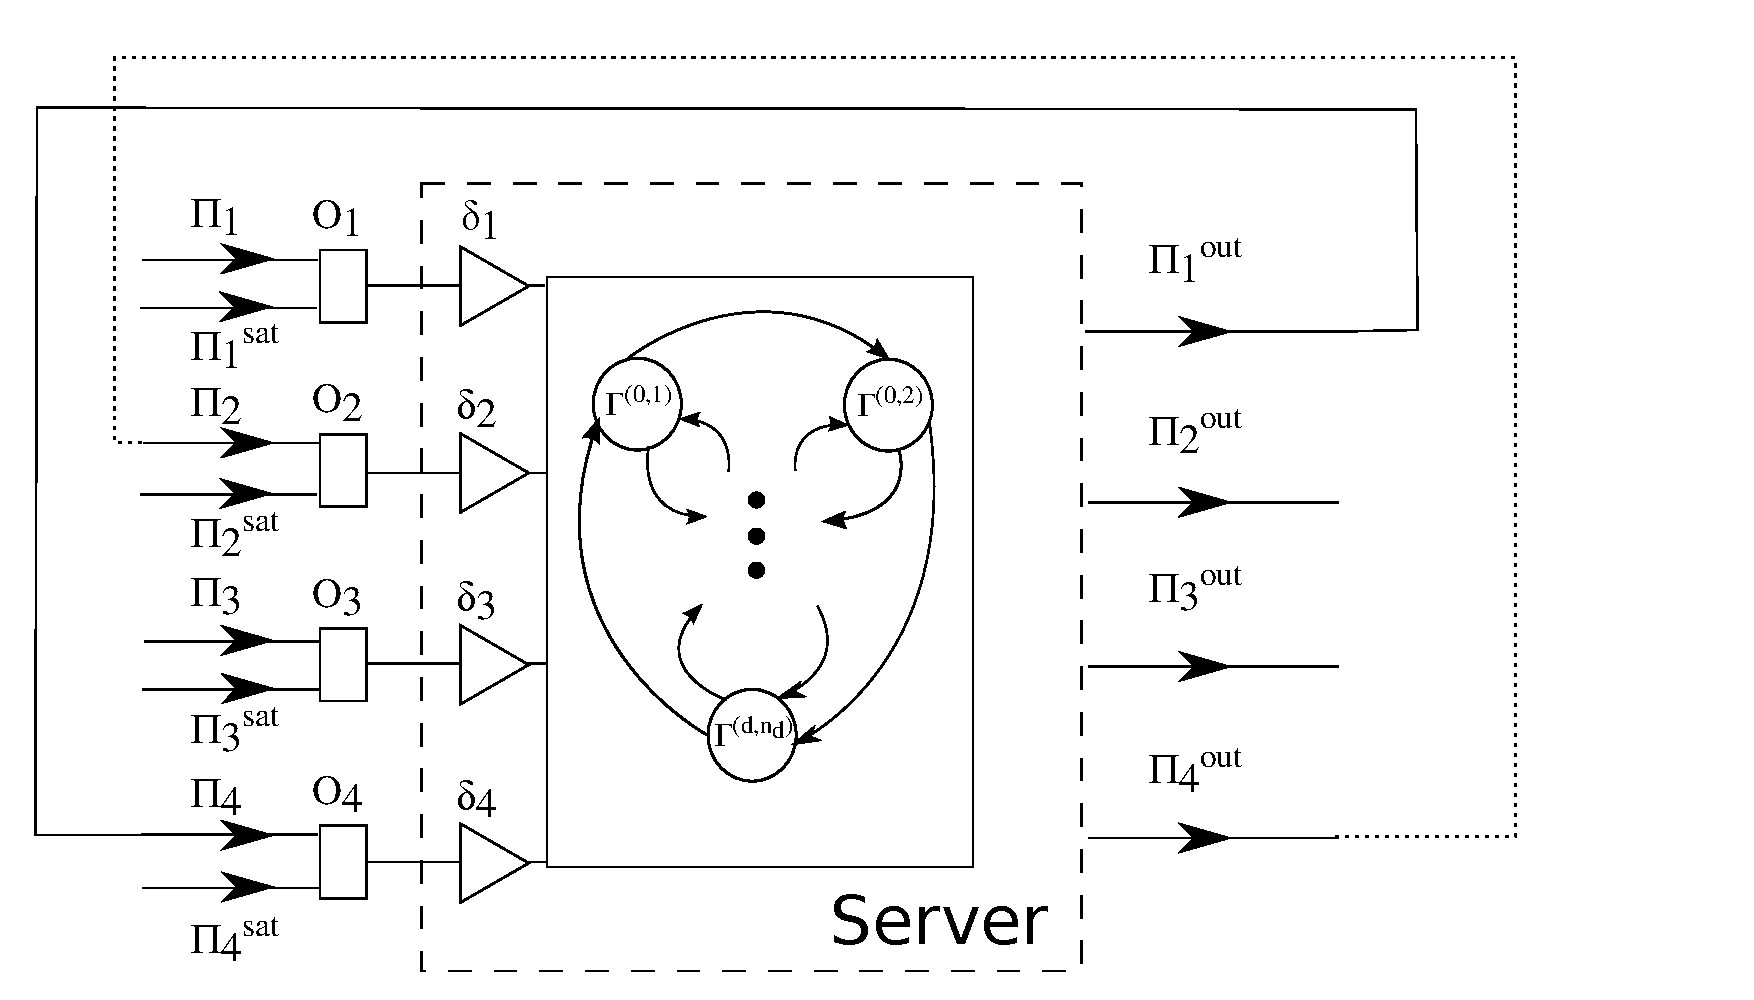
\includegraphics[width=13cm]{SystemScheme.pdf}
    \caption {Рис.~1: Схема СМО как управляющей кибернетической системы}
\end{figure}

В работе~[2] были выделены информация, координаты и функция данной системы. Это
позволило конструктивно задать последовательности случайных величин и случайных
элементов, описывающих диксретную временную шкалу наблюдения и состояния всех
блоков схемы. В частности, в качестве дискретной временной шкалы выбрана
последовательность $\tau_0=0$, $\tau_1$, $\tau_2$, $\ldots$ моментов смены
состояния обслуживающего устройства. Обозначим $\Gamma_i\in\Gamma$, $i=1$, $2$,
\ldots{} состояние обслуживающего устройства в течение времени
$\left(\tau_{i-1};\tau_i\right]$ и $\Gamma_0\in \Gamma$ его состояние в момент
времени $\tau_0$ и пусть $\varkappa_{j,i} \in \mathbb{Z}_+ $ "--- количество
требований в очереди $O_j$ в момент времени $\tau_i$, , $i\geqslant 0$.  
Было доказано, что стохастическая последовательность $\{(\Gamma_i,
\varkappa_{1,i}, \varkappa_{2,i}, \varkappa_{3,i}, \varkappa_{4,i}); i=0, 1,
\ldots\}$ является однородной цепью Маркова. Свойства последовательности $\{(\Gamma_i,\varkappa_{3,i}); i \geqslant 0\}$ изучены в работах~[1,3].


\Subtitle{Основной результат}

В данной работе мы рассматриваем последовательность  
\[
\{(\Gamma_i,
\varkappa_{1,i},\varkappa_{3,i}); i \geqslant 0\}. \tag{1} 
\]

\noindent{\bfseries Теорема 1.}  {\itshape 
  Стохастическая последовательность~(1)
  при заданном распределении элемента $(\Gamma_0, \varkappa_{1,0},
  \varkappa_{2,0}, \varkappa_{3,0}, \varkappa_{4,0})$ является однородной цепью
  Маркова.  
}

\smallskip

\noindent
{\bfseries Теорема 2.}
{\itshape
Для того, чтобы марковская цепь~(1) имела стационарное распределение,  достаточно выполнения неравенства 
$$
\min_{\substack{k=\overline{1,d}\\ j=1,3}} { \frac{\sum_{r = 1}^{n_k} \ell(k,r,j) }{\lambda_j f_j'(1) \sum_{r=1}^{n_k} T^{(k,r)} }}>1.
$$
}


\begin{ptkreferences}
\selectlanguage{english}
\item
Kocheganov~V.\,M., Zorine~A.\,V. Low-Priority Queue and Server’s Steady-State
Existence in a Tandem Under Prolongable Cyclic Service~//  Distributed Computer
and Communication Networks. DCCN 2016. Communications in Computer and
Information Science (Vishnevskiy V., Samouylov K., Kozyrev D. (eds)). ---
Springer, Cham.--- V.\,678. --- 2016. --- pp.\,210--221. 
\selectlanguage{russian}
\item
Кочеганов~В.\,М., Зорин~А.\,В. Вероятностная модель тандема систем массового обслуживания с циклическим управлением с продлением // Теория вероятностей, случайные процессы, математическая статистика и приложения: материалы Междунар. науч. конф., посвящ. 80-летию проф., д-ра физ.-мат. наук Г.\,А. Медведева, Минск "--- 23–26 февр. 2015. "--- С.\,94--99.

\item
Kocheganov~V.\,M., Zorine~A.\,V. Low-priority queue fluctuations in tandem of queueing systems under cyclic control with prolongations // Распределенные компьютерные и телекоммуникационнные сети: управление, вычисление, связь (DCCN-2015) : материалы Восемнадцатой междунар. науч. конфер., 19–22 окт. 2015 г., Москва: / Ин-т проблем упр. им. В.А. Трапезникова Рос. акад. наук ; под общ. ред. В.М. Вишневского. —М.: ИПУ РАН "--- 2015. "--- С.~517--524.


\end{ptkreferences}

\end{ptkarticle}    

%%% Local Variables:
%%% Сoding: cp1251
%%% TeX-PDF-mode: t
%%% TeX-master: "ptk18main.tex"
%%% End: